\documentclass{subfiles}

\begin{document}

    \chapter{Planificación}
    \label{chap:planificacion}

        \section{Planificación inicial}
        \label{sec:planificacion_inicial}

        \subsection{Metodología}
        \label{sec:metodologia}
        
        {Debido a la capacidad de adaptación ante nuevos requisitos y a la posibilidad de generar nuevas entregas a la mayor brevedad posible utilizando metodologías ágiles, se ha optado por esta preferiblemente sobre otras \cite{agilewebsite}. De esta manera, las partes interesadas serían capaces de ver en periodos cortos de tiempo avances en el proyecto que supongan un cambio importante. Es importante mencionar que, debido a que el equipo de desarrollo contaba solamente con una persona, no se ha aplicado el marco de trabajo \textit{Scrum}, puesto que este está planteado para equipos más grandes.}
        
        \paragraph{}
        {Para centrar el trabajo en el menor número de tareas posibles al mismo tiempo, y favorecer la visibilidad del estado de las tareas y del proyecto, se ha decidido utilizar una adaptación de la metodología \Kanban\cite{web:kanban}, una subcategoría de gestión ágil de proyectos centrada en el uso de los tableros homónimos. La idea de usar esta metodología surgió después de atender a una charla de Pablo Santos en la Escuela de Ingeniería Informática en la Universidad de Valladolid \cite{web:pablosantos}, donde nos explicó los diferentes proyectos que dirigió, así como las metodologías que aplicó para liderarlos. En el momento de la charla, explicó como la metodología \Kanban le permitía dar más visibilidad a las tareas en proceso así como ver el flujo de trabajo, tal y como relata en su libro, \textit{Version Control, DevOps and Agile Development with Plastic SCM} \cite{book:santos_pablo_versioncontrol}.}

        \begin{figure}
        \centering
        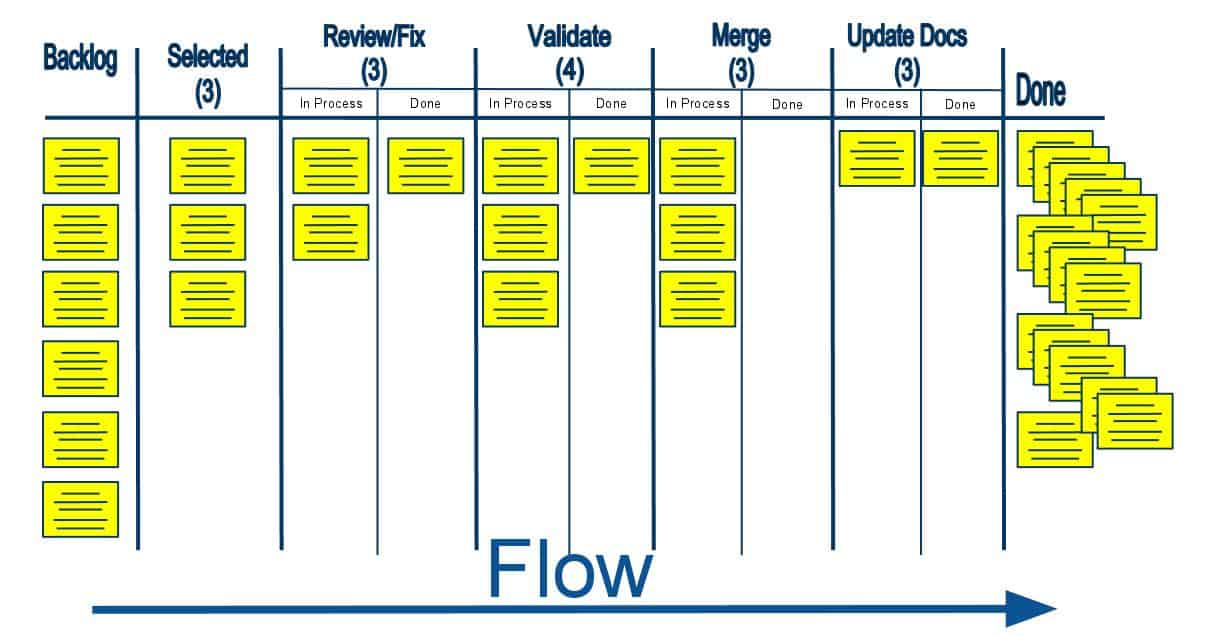
\includegraphics[width=0.8\textwidth]{kanbanboard}
        \caption{Ejemplo de flujo en un tablero \Kanban. Fuente: \citetitle{web:mulesoft_kanban}.}
        \label{fig:kanbanboard}
        \end{figure}

        \paragraph{}
        {Según David Anderson, el ingeniero de Microsoft que aplicó esta metodología por primera vez a proyectos informáticos \cite{book:anderson_david_kanban}, los tableros \Kanban contienen cinco elementos característicos: señales visuales, columnas, límites de trabajo en curso, punto de compromiso y punto de entrega.}

        \begin{itemize}
            \item {\textbf{Señales visuales}: todo el trabajo, junto con su estado actual, debe ser visible de un solo vistazo. Esta metodología utiliza las tarjetas como representación de tareas únicas que, en combinación con las columnas, nos revelarán el flujo de trabajo y el estado actual de este último, todo esto sin abandonar la filosofía de <<información visual>> de \Kanban.}
            \item {\textbf{Columnas}: representan el estado de la tarea en el flujo de trabajo. Los tableros más sencillos suelen utilizar 3 columnas (\textit{pendiente}, \textit{en curso}, \textit{finalizado}), aunque cada equipo puede organizar su flujo de trabajo a placer. Así, para indicar la evolución de cada tarea, las tarjetas avanzarán por diferentes columnas hasta su finalización, yendo idealmente siempre hacia la derecha. En su charla, Pablo Santos llegó a indicar que cada empleado tenía su propia columna de <<trabajo en curso>> para visibilizar de manera más eficaz con qué tarea se encontraba cada empleado.}
            \item {\textbf{Límites de trabajo en curso}: las columnas que indican el trabajo en curso deben tener un límite establecido de tarjetas en ella. Este, según las buenas prácticas, suele ser menor que el número de miembros del equipo para que, si un miembro termina una tarea y no puede comenzar otra por este límite, se dedique a la revisión de código o a apoyar a otros compañeros a finalizar tareas que puedan haberse atascado. Así, cuando una de estas columnas alcanza su límite de tarjetas, el equipo debe aplicar todo su esfuerzo en estas para lograr que avancen. Esta es la forma visual que tiene \Kanban de mostrar al equipo que se está intentando asumir demasiado trabajo y de avisar de posibles cuellos de botella.}
            \item {\textbf{Punto de compromiso}: \Kanban trabaja con una pila de tareas por desarrollar, comúnmente llamada \textit{backlog}, que va creciendo según van apareciendo nuevas necesidades o requisitos. Cada vez que una de esas tareas sale de la columna de tareas pendientes, el miembro del equipo se <<compromete>> a terminar esa tarea en el menor tiempo posible. El momento de inicio de cada tarea se denomina por esto <<punto de compromiso>>}
            \item {\textbf{Punto de entrega}: es el momento en que una tarjeta se convierte en un trabajo completado y, por tanto, está ya en manos del cliente o del producto final. El tiempo entre el punto de compromiso y el punto de entrega se denomina <<plazo>>, y la intención de la forma de trabajar con \Kanban es que ese plazo sea el menor posible.}
        \end{itemize}
        
        \paragraph{}
        {Al ser un proyecto de innovación dentro de la empresa, los requisitos iban surgiendo según íbamos encontrando nueva información al respecto. De esta manera, durante reuniones semanales se comentaba el avance del proyecto, así como las nuevas tareas a incorporar junto con su prioridad, procurando siempre no solapar unas tareas con otras. Esto implica que, al final de dichas reuniones, generalmente se ampliaba el \textit{backlog} del tablero \Kanban, siendo común que en cada reunión surgiesen una o dos nuevas tarjetas. En este aspecto, la aplicación de esta metodología se ajustaba mejor que otras metodologías al trabajo realizado, debido a que toda tarea terminada podía ser subida en <<su propia \textit{release}>>. En ese aspecto, \textit{Scrum} es mucho más estricto, dependiendo de \textit{sprints}. Esta última además es muy dependiente de reuniones (planificaciones de \textit{sprints}, reuniones diarias, revisiones de \textit{sprints}, retrospectivas), que parecen perder utilidad cuando el equipo está reducido a tres personas que, además, mantienen el contacto en todo momento. Se planteó también utilizar un modelo de prototipado de Software, debido a que se desconocía el resultado del producto final y de los requisitos del proyecto. Sin embargo, la investigación previa de los sistemas existentes permitió aclarar muchos aspectos del producto y establecer un plan de ruta que, aunque se pudiese desviar, permitiría planear con mayor o menor antelación las tareas necesarias.}

        \paragraph{}
        A pesar de que no había roles específicos definidos dentro del propio proyecto, sí podían diferenciarse algunos relacionados con la gestión de proyectos asociados a los tres miembros del equipo:
        \begin{itemize}
            \item \textbf{Álvaro Aparicio} procuraba que el desarrollo del producto fuese en todo momento beneficioso para la empresa, dando una serie de ideas generales para que el resto del equipo las diese forma y las llevara a la práctica. Él se dedicaba también a informar al CEO de la empresa de los avances, así como de tratar con otros sectores en caso de necesitar información o ayuda. Su rol sería, en este equipo, el \textit{Product Owner}.
            
            \item \textbf{Alberto Sáenz} tomaba decisiones sobre avances, procuraba hacer de puente entre las ideas generales propuestas por el primer miembro y las tareas técnicas a desarrollar y gestionaba y coordinaba el proyecto así como sus tiempos. Por su implicación, su rol sería \textit{Project Manager}, aunque también haría las veces de \textit{Team Lead} debido a su gestión del trabajo de los miembros.
            
            \item Por último, \textbf{mi posición}, dedicada principalmente al desarrollo, a aprender sobre las nuevas tecnologías y a investigar sobre las mismas, se acercaría principalmente al rol de desarrollador, pero al ser necesario un conocimiento intensivo de las tecnologías aplicadas y su interpretación para el resto del equipo, también se podría aplicar \textit{Tech lead}.
        \end{itemize}

        \subsection{Organización del tiempo}
        \label{sec:organizacion_del_tiempo}

        Este proyecto se planteó para ser desarrollado desde el 4 de octubre de 2021, siendo su fecha de finalización el 30 de septiembre de 2022. Esto hace 250 días laborables, de los cuáles, para compaginar este con otros proyectos, se planteó dedicar al día un 25\% de la jornada total semanal, lo que hace unas 500 horas dedicadas a este proyecto. El proyecto está dividido en 3 grandes actividades, cada una de ellas dividida en subelementos a completar, tal y como se describe en la tabla \ref{tab:cronograma_del_proyecto}.

        %%%%%%%%%%%%%%%%%%%%
        %%%%%%%% TABLE START
        %%%%%%%%%%%%%%%%%%%%
\begin{landscape}
\begin{table}%[h]
\begin{tabular}{|ll|ccc|ccccccccc|}
\hline
\multicolumn{2}{|l|}{}                                                        & \multicolumn{3}{c|}{2021}                                                                                                & \multicolumn{9}{c|}{2022}                                                                                                                                                                                                                                                                                                                                                                                                \\ \hline
\multicolumn{2}{|l|}{}                                                        & \multicolumn{1}{c|}{Oct}                      & \multicolumn{1}{c|}{Nov}                      & Dic                      & \multicolumn{1}{c|}{Ene}                      & \multicolumn{1}{c|}{Feb}                      & \multicolumn{1}{c|}{Mar}                      & \multicolumn{1}{c|}{Abr}                      & \multicolumn{1}{c|}{May}                      & \multicolumn{1}{c|}{Jun}                      & \multicolumn{1}{c|}{Jul}                      & \multicolumn{1}{c|}{Ago}                      & Sep                      \\ \hline
\multicolumn{2}{|l|}{1. Prueba de Concepto (PoC)}                             & \multicolumn{1}{c|}{\cellcolor[HTML]{656565}} & \multicolumn{1}{c|}{\cellcolor[HTML]{656565}} & \cellcolor[HTML]{656565} & \multicolumn{1}{c|}{}                         & \multicolumn{1}{c|}{}                         & \multicolumn{1}{c|}{}                         & \multicolumn{1}{c|}{}                         & \multicolumn{1}{c|}{}                         & \multicolumn{1}{c|}{}                         & \multicolumn{1}{c|}{}                         & \multicolumn{1}{c|}{}                         &                          \\ \hline
              & 1.1 Concepto y estudio de su viabilidad                       & \multicolumn{1}{c|}{\cellcolor[HTML]{9B9B9B}} & \multicolumn{1}{c|}{}                         &                          & \multicolumn{1}{c|}{}                         & \multicolumn{1}{c|}{}                         & \multicolumn{1}{c|}{}                         & \multicolumn{1}{c|}{}                         & \multicolumn{1}{c|}{}                         & \multicolumn{1}{c|}{}                         & \multicolumn{1}{c|}{}                         & \multicolumn{1}{c|}{}                         &                          \\ \hline
              & 1.2 Estudio y especificación de requisitos mínimo             & \multicolumn{1}{c|}{\cellcolor[HTML]{9B9B9B}} & \multicolumn{1}{c|}{}                         &                          & \multicolumn{1}{c|}{}                         & \multicolumn{1}{c|}{}                         & \multicolumn{1}{c|}{}                         & \multicolumn{1}{c|}{}                         & \multicolumn{1}{c|}{}                         & \multicolumn{1}{c|}{}                         & \multicolumn{1}{c|}{}                         & \multicolumn{1}{c|}{}                         &                          \\ \hline
              & 1.3 Diseño de la arquitectura de la PoC                       & \multicolumn{1}{c|}{\cellcolor[HTML]{9B9B9B}} & \multicolumn{1}{c|}{\cellcolor[HTML]{9B9B9B}} &                          & \multicolumn{1}{c|}{}                         & \multicolumn{1}{c|}{}                         & \multicolumn{1}{c|}{}                         & \multicolumn{1}{c|}{}                         & \multicolumn{1}{c|}{}                         & \multicolumn{1}{c|}{}                         & \multicolumn{1}{c|}{}                         & \multicolumn{1}{c|}{}                         &                          \\ \hline
              & 1.4 Desarrollo de la PoC                                      & \multicolumn{1}{c|}{}                         & \multicolumn{1}{c|}{\cellcolor[HTML]{9B9B9B}} & \cellcolor[HTML]{9B9B9B} & \multicolumn{1}{c|}{}                         & \multicolumn{1}{c|}{}                         & \multicolumn{1}{c|}{}                         & \multicolumn{1}{c|}{}                         & \multicolumn{1}{c|}{}                         & \multicolumn{1}{c|}{}                         & \multicolumn{1}{c|}{}                         & \multicolumn{1}{c|}{}                         &                          \\ \hline
\multicolumn{2}{|l|}{2. Diseño y desarrollo del Producto Mínimo Viable (MVP)} & \multicolumn{1}{c|}{}                         & \multicolumn{1}{c|}{}                         & \cellcolor[HTML]{656565} & \multicolumn{1}{c|}{\cellcolor[HTML]{656565}} & \multicolumn{1}{c|}{\cellcolor[HTML]{656565}} & \multicolumn{1}{c|}{\cellcolor[HTML]{656565}} & \multicolumn{1}{c|}{}                         & \multicolumn{1}{c|}{}                         & \multicolumn{1}{c|}{}                         & \multicolumn{1}{c|}{}                         & \multicolumn{1}{c|}{}                         &                          \\ \hline
              & 2.1 Análisis de especificaciones del MVP                      & \multicolumn{1}{c|}{}                         & \multicolumn{1}{c|}{}                         & \cellcolor[HTML]{9B9B9B} & \multicolumn{1}{c|}{}                         & \multicolumn{1}{c|}{}                         & \multicolumn{1}{c|}{}                         & \multicolumn{1}{c|}{}                         & \multicolumn{1}{c|}{}                         & \multicolumn{1}{c|}{}                         & \multicolumn{1}{c|}{}                         & \multicolumn{1}{c|}{}                         &                          \\ \hline
              & 2.2 Diseño y arquitectura del MVP                             & \multicolumn{1}{c|}{}                         & \multicolumn{1}{c|}{}                         &                          & \multicolumn{1}{c|}{\cellcolor[HTML]{9B9B9B}} & \multicolumn{1}{c|}{\cellcolor[HTML]{9B9B9B}} & \multicolumn{1}{c|}{}                         & \multicolumn{1}{c|}{}                         & \multicolumn{1}{c|}{}                         & \multicolumn{1}{c|}{}                         & \multicolumn{1}{c|}{}                         & \multicolumn{1}{c|}{}                         &                          \\ \hline
              & 2.3 Desarrollo incremental del MVP                            & \multicolumn{1}{c|}{}                         & \multicolumn{1}{c|}{}                         &                          & \multicolumn{1}{c|}{}                         & \multicolumn{1}{c|}{\cellcolor[HTML]{9B9B9B}} & \multicolumn{1}{c|}{\cellcolor[HTML]{9B9B9B}} & \multicolumn{1}{c|}{}                         & \multicolumn{1}{c|}{}                         & \multicolumn{1}{c|}{}                         & \multicolumn{1}{c|}{}                         & \multicolumn{1}{c|}{}                         &                          \\ \hline
              & 2.4 Integración, pruebas y validación del MVP                 & \multicolumn{1}{c|}{}                         & \multicolumn{1}{c|}{}                         &                          & \multicolumn{1}{c|}{}                         & \multicolumn{1}{c|}{}                         & \multicolumn{1}{c|}{\cellcolor[HTML]{9B9B9B}} & \multicolumn{1}{c|}{}                         & \multicolumn{1}{c|}{}                         & \multicolumn{1}{c|}{}                         & \multicolumn{1}{c|}{}                         & \multicolumn{1}{c|}{}                         &                          \\ \hline
\multicolumn{2}{|l|}{3. Desarrollo del Producto Final (FP)}                   & \multicolumn{1}{c|}{}                         & \multicolumn{1}{c|}{}                         &                          & \multicolumn{1}{c|}{}                         & \multicolumn{1}{c|}{}                         & \multicolumn{1}{c|}{\cellcolor[HTML]{656565}} & \multicolumn{1}{c|}{\cellcolor[HTML]{656565}} & \multicolumn{1}{c|}{\cellcolor[HTML]{656565}} & \multicolumn{1}{c|}{\cellcolor[HTML]{656565}} & \multicolumn{1}{c|}{\cellcolor[HTML]{656565}} & \multicolumn{1}{c|}{\cellcolor[HTML]{656565}} & \cellcolor[HTML]{656565} \\ \hline
              & 3.1 Análisis del FP                                           & \multicolumn{1}{c|}{}                         & \multicolumn{1}{c|}{}                         &                          & \multicolumn{1}{c|}{}                         & \multicolumn{1}{c|}{}                         & \multicolumn{1}{c|}{\cellcolor[HTML]{9B9B9B}} & \multicolumn{1}{c|}{\cellcolor[HTML]{9B9B9B}} & \multicolumn{1}{c|}{}                         & \multicolumn{1}{c|}{}                         & \multicolumn{1}{c|}{}                         & \multicolumn{1}{c|}{}                         &                          \\ \hline
              & 3.2 Diseño y desarrollo incremental                           & \multicolumn{1}{c|}{}                         & \multicolumn{1}{c|}{}                         &                          & \multicolumn{1}{c|}{}                         & \multicolumn{1}{c|}{}                         & \multicolumn{1}{c|}{}                         & \multicolumn{1}{c|}{\cellcolor[HTML]{9B9B9B}} & \multicolumn{1}{c|}{\cellcolor[HTML]{9B9B9B}} & \multicolumn{1}{c|}{\cellcolor[HTML]{9B9B9B}} & \multicolumn{1}{c|}{\cellcolor[HTML]{9B9B9B}} & \multicolumn{1}{c|}{\cellcolor[HTML]{9B9B9B}} & \cellcolor[HTML]{9B9B9B} \\ \hline
              & 3.3 Integración, pruebas y despliegue del FP                  & \multicolumn{1}{c|}{}                         & \multicolumn{1}{c|}{}                         &                          & \multicolumn{1}{c|}{}                         & \multicolumn{1}{c|}{}                         & \multicolumn{1}{c|}{}                         & \multicolumn{1}{c|}{}                         & \multicolumn{1}{c|}{}                         & \multicolumn{1}{c|}{}                         & \multicolumn{1}{c|}{}                         & \multicolumn{1}{c|}{\cellcolor[HTML]{9B9B9B}} & \cellcolor[HTML]{9B9B9B} \\ \hline
\end{tabular}
\caption{Cronograma del proyecto}
\label{tab:cronograma_del_proyecto}
\end{table}
\end{landscape}
        %%%%%%%%%%%%%%%%%%%%
        %%%%%%%% TABLE END
        %%%%%%%%%%%%%%%%%%%%

        \subsection{Gestión de riesgos}
        \label{sec:gestion_de_riesgos}
        Durante el proyecto, hay una serie de imprevistos que pueden dificultar el avance de este. Debido al carácter académico y corporativo de este, se han planteado una serie de riesgos que no coinciden completamente con los más comunes en la gestión de riesgos y que pueden considerarse como algunos de los más importantes en los que centrarse. Idealmente, en un proyecto, se suelen plantear 10 riesgos en los que centrarse, pero según el libro \citetitle{book:hughes_bob_softwareprojectManagement} \cite{book:hughes_bob_softwareprojectManagement}, este número es recomendable para proyectos que no se consideran pequeños, siendo recomendable para estos reducir este número.

        \paragraph{}
        Para categorizar los riesgos seleccionados, se ha decidido utilizar una matriz de exposición al riesgo como el de la tabla \ref{tab:exposicion_al_riesgo}, donde la probabilidad se explica en la tabla \ref{tab:probabilidades_de_riesgos} y el impacto en la tabla \ref{tab:impacto_de_riesgos}.


%%%%%%%%%%%%%%%%%%%%%%%%%%%%%%%%
%% TABLA DE EXPOSICION AL RIESGO
%%%%%%%%%%%%%%%%%%%%%%%%%%%%%%%%
\begin{table}[h]
\centering
\begin{tabular}{cccccc}
                         &                                    & \multicolumn{4}{c}{Probabilidad}                                                                                                             \\
                         &                                    & Bajo                          & Moderado                           & Significativo                      & Alto                               \\ \cline{3-6} 
\multirow{4}{*}{\begin{turn}{90}Impacto\end{turn}} & \multicolumn{1}{c|}{Alto}          & \multicolumn{1}{c|}{Moderado} & \multicolumn{1}{c|}{Significativo} & \multicolumn{1}{c|}{Alto}          & \multicolumn{1}{c|}{Alto}          \\ \cline{3-6} 
                         & \multicolumn{1}{c|}{Significativo} & \multicolumn{1}{c|}{Bajo}     & \multicolumn{1}{c|}{Moderado}      & \multicolumn{1}{c|}{Significativo} & \multicolumn{1}{c|}{Alto}          \\ \cline{3-6} 
                         & \multicolumn{1}{c|}{Moderado}      & \multicolumn{1}{c|}{Bajo}     & \multicolumn{1}{c|}{Moderado}      & \multicolumn{1}{c|}{Moderado}      & \multicolumn{1}{c|}{Significativo} \\ \cline{3-6} 
                         & \multicolumn{1}{c|}{Bajo}          & \multicolumn{1}{c|}{Bajo}     & \multicolumn{1}{c|}{Bajo}          & \multicolumn{1}{c|}{Bajo}          & \multicolumn{1}{c|}{Moderado}      \\ \cline{3-6} 
\end{tabular}
\caption{Tablero de exposición al riesgo utilizado. Fuente: \citetitle{web:projectriskmanagement_doessizereallymatter}}
\label{tab:exposicion_al_riesgo}
\end{table}
%%%%%%%%%%%%%%%%%%%%%%%%%%
%% TABLA DE PROBABILIDADES
%%%%%%%%%%%%%%%%%%%%%%%%%%

\begin{table}[h]
\centering
\begin{tabular}{ll}
\hline
\textbf{Nivel de probabilidad} & \textbf{Rango}                       \\ \hline
Alto                           & Probabilidad mayor del 50\%          \\ \hline
Significativo                  & Probabilidad entre el 30\% y el 50\% \\ \hline
Moderado                       & Probabilidad entre el 10\% y el 29\% \\ \hline
Bajo                           & Probabilidad menor del 10\%          \\ \hline
\end{tabular}
\caption{Niveles de probabilidad utilizados. Fuente: \citetitle{book:hughes_bob_softwareprojectManagement}.}
\label{tab:probabilidades_de_riesgos}
\end{table}

%%%%%%%%%%%%%%%%%%%%%%%
%%%%%% TABLA DE IMPACTO
%%%%%%%%%%%%%%%%%%%%%%%
\begin{table}[h]
\centering
\begin{tabular}{ll}
\hline
\textbf{Nivel de impacto} & \textbf{Rango}                              \\ \hline
Alto                      & Gasto superior al 30\% presupuestado        \\ \hline
Significativo             & Gasto entre el 20\% y el 30\% presupuestado \\ \hline
Moderado                  & Gasto entre el 10\% y el 19\% presupuestado \\ \hline
Bajo                      & Gasto inferior al 10\% presupuestado        \\ \hline
\end{tabular}
\caption{Niveles de impacto utilizados. Fuente: \citetitle{book:hughes_bob_softwareprojectManagement}.}
\label{tab:impacto_de_riesgos}
\end{table}

        Los riesgos a tener en cuenta para este proyecto se van a presentar en dos tablas. La primera de ellas, la tabla \ref{tab:presentacion_riesgos}, presentará dichos riesgos junto con su código, su nombre, su descripción, su probabilidad, su impacto y la exposición resultante del cálculo a través de estos dos últimos valores.

%%%%%%%%%%%%%%%%%%%%%%%%%%
%% PRESENTACIÓN DE RIESGOS
%%%%%%%%%%%%%%%%%%%%%%%%%%

\begin{longtblr}[
  caption = {Presentación de los riesgos},
  label = {tab:presentacion_riesgos},
]{
  width = \linewidth,
  colspec = {Q[60]Q[161]Q[499]Q[73]Q[70]Q[70]},
  hlines,
  vlines,
}
\textbf{Cód.} & \textbf{Nombre} & \textbf{Descripción} & \textbf{Prob.} & \textbf{Imp.} & \textbf{Exp.}\\
RSK1 & Cambios en el alcance del proyecto & La planificación original deja de corresponderse con la actual debido a falta de tareas no previstas en el análisis, o por cambios en el alcance tras las investigaciones del proyecto. & Sign. & Sign. & Sign.\\
RSK2 & Estimación del tiempo inadecuada & La estimación del tiempo de cada tarea resulta inferior a la real y la fecha de finalización de proyecto resulta imposible de cumplir & Sign. & Sign. & Sign.\\
RSK3 & Pérdida del progreso del proyecto & Debido a ataques o a fallos de sistema, se pierde una parte o la totalidad de los ficheros o información del proyecto & Bajo & Alto & Mod.\\
RSK4 & La tecnología utilizada no ofrece la calidad esperada & Tras implementar la prueba de concepto, la calidad de la tecnología aplicada es menor de la esperada & Mod. & Sign. & Mod.\\
RSK5 & Falta de experiencia con las librerías a utilizar & Las librerías a implementar en la aplicación son demasiado complejas y requieren más tiempo del previsto para dominarlos & Mod. & Sign. & Mod.\\
RSK6 & Documentación del software a utilizar deficiente o mínimo & Las librerías, las herramientas y el lenguaje de programación a utilizar en el proyecto no resultan de la ayuda adecuada para resolver las dudas o problemas que puedan surgir durante el proyecto & Mod. & Mod. & Mod.\\
RSK7 & Baja o ausencia del personal & El personal se ausenta del proyecto durante un tiempo significativo por causas de fuerza mayor & Bajo & Mod. & Bajo\\
RSK8 & Pérdida del hardware del proyecto & Debido a fallos en los equipos o en los dispositivos móviles utilizados para desarrollar y probar el proyecto, alguno o todos estos dejan de funcionar & Bajo & Mod. & Bajo\\
RSK9 & Actualizaciones de las librerías utilizadas & Las librerías implementadas en el proyecto reciben actualizaciones mayores que cambian parte de su implementación & Bajo & Mod. & Bajo
\end{longtblr}

%%%%%%%%%%%%%%%%%%%%%%%%%%%%%%
%% FIN PRESENTACIÓN DE RIESGOS
%%%%%%%%%%%%%%%%%%%%%%%%%%%%%%

        \paragraph{}
        Una vez presentados los riesgos se muestra la tabla \ref{tab:mitigacion_contingencia_riesgos}, donde cada riesgo aparece acompañado por código, su nombre, su plan de mitigación y su plan de contingencia. Aquí, los planes de mitigación intentan minimizar el daño del riesgo mientras este no se haya cumplido, mientras que los planes de contingencia abordan el riesgo en caso de haberse cumplido.

%%%%%%%%%%%%%%%%%%%%%%%%%%%%%%%%%%%%%%%
%% MITIGACION Y CONTINGENCIA DE RIESGOS
%%%%%%%%%%%%%%%%%%%%%%%%%%%%%%%%%%%%%%%

% \usepackage{tabularray}
\begin{longtblr}[
  caption = {Planes de mitigación y contingencia sobre los distintos riesgos},
  label = {tab:mitigacion_contingencia_riesgos},
]{
  width = \linewidth,
  colspec = {Q[71]Q[156]Q[367]Q[341]},
  hlines,
  vlines,
}
\textbf{Cód.} & \textbf{Nombre} & \textbf{Mitigación} & \textbf{Contingencia}\\
RSK1 & Cambios en el alcance del proyecto & Revisar semanalmente el alcance y necesidades del proyecto en relación al producto en el momento & Replanificar las tareas del proyecto, analizando cuáles son las nuevas tareas más prioritarias para obtener el producto mínimo viable\\
RSK2 & Estimación del tiempo inadecuada & Revisar semanalmente las tareas pendientes y analizar su complejidad en relación con la experiencia obtenida sobre el mismo proyecto & Modificar y aumentar la dedicación semanal al proyecto para reducir la fecha de entrega\\
RSK3 & Pérdida del progreso del proyecto & Realizar copias de seguridad tras cada cambio en un sistema de control de versiones & Buscar opciones o software de recuperación de datos. En su defecto, reducir y replanificar los objetivos del proyecto.\\
RSK4 & La tecnología utIlizada no ofrece la calidad esperada & Revisar durante la planificación casos prácticos en los que se hayan utilizado las librerías a utilizar & Buscar un nuevo software que reemplace el de baja calidad y replanificar objetivos dando prioridad a las tareas necesarias para el producto mínimo viable\\
RSK5 & Falta de experiencia con las librerías a utilizar & Aumentar la dedicación a formación e investigación de las tecnologías utilizadas & Añadir personal de apoyo en el desarrollo del producto\\
RSK6 & Documentación del software a utilizar deficiente o mínimo & Aumentar la dedicación a formación e investigación de las tecnologías utilizadas y revisar tutoriales profesionales previamente al desarrollo del producto & Buscar información relativa a las consultas necesarias en foros dedicados o en fuentes alternativas\\
RSK7 & Baja o ausencia del personal & Plantear las tareas con un "buffer" que pueda compensar la posible ausencia del personal & Replanificar el proyecto dando prioridad a las tareas necesarias para el producto mínimo viable\\
RSK8 & Pérdida del hardware del proyecto & Asegurar el almacenamiento de todo lo necesario para el proyecto en la nube o en copias de seguridad para poder continuar con distintos dispositivos & Adquirir nuevo hardware de desarrollo\\
RSK9 & Actualizaciones de las librerías utilizadas & Revisar mensualmente novedades sobre el software utilizado para prever posibles cambios & Estudiar los cambios en la actualización del software y pruebas sobre el producto desarrollado para comprobar que todo funcione correctamente
\end{longtblr}

%%%%%%%%%%%%%%%%%%%%%%%%%%%%%%%%%%%%%%%%%%%
%% FIN MITIGACION Y CONTINGENCIA DE RIESGOS
%%%%%%%%%%%%%%%%%%%%%%%%%%%%%%%%%%%%%%%%%%%

        \subsection{Recursos}
        \label{sec:recursos}

        Dentro del proyecto se han utilizado principalmente los recursos ofrecidos por la empresa, a mayores de una serie de recursos de uso libre o de posesión propia. Todos estos se pueden desglosar en hardware y software:

        \begin{itemize}
            \item \textbf{Hardware}: se ha utilizado para el desarrollo del código el equipo ofrecido por la empresa (\textit{Dell Vostro 3400}), a mayores del dispositivo móvil personal para pruebas de desarrollo (\textit{Xiaomi Redmi Note 9 Pro}). También, como apoyo al desarrollo, se incluyen los periféricos ofrecidos por la empresa (pantalla, teclado y ratón) a mayores del sistema de internet inalámbrico montado en las oficinas. También entran en esta categoría el cable de carga del ordenador portátil y el cable USB tipo C para conectar el móvil al portátil.
            \item \textbf{Software}: comenzando por el sistema operativo, ofrecido por la empresa en conjunto con el equipo, este es un \textit{Windows 10 Pro}. En el dispositivo móvil, se ha utilizado en sistema operativo \android. En ambos sistemas operativos se ha instalado el navegador \googlechrome, cada uno en su respectiva versión. Para el desarrollo, se ha utilizado el IDE \eclipse en su versión para desarrollo web para soportar el lenguaje \js. Todo el código ha sido almacenado en \github, y para las cargas se ha utilizado \gitkraken. Para el desarrollo de la memoria se ha utilizado \overleaf, para la generación de diagramas se ha utilizado \drawio y para la creación de objetos 3D se ha utilizado tanto \blender como \makehuman. Por último, se ha utilizado \aws para poder ubicar la aplicación en un servidor y para poder utilizar sus servicios web.
        \end{itemize}

        No conviene olvidar como recursos humanos al equipo formado por Álvaro Aparicio, Alberto Sáenz y Miguel Bayón, además de todo el equipamiento básico de trabajo que ofrece una empresa como las oficinas, aspectos básicos atados a esta (luz, gas y agua), silla y mesa, entre otros.

        \subsection{Estimación de costes}
        \label{sec:estimacion_de_costes}

        \section{Planificación final}
        \label{sec:planificacion_final}

\end{document}